%!TEX root = ../documentation.tex

\chapter{Einsatzbereiche}
\section{Norbert - Wie kommt er in das Leben eines Studierenden?}
Norbert - Your StudyBuddy ist eine Anwendung zum Optimieren des Studienalltags, doch wie werden die Studierenden darauf aufmerksam?
Um Norbert bekannt zu machen und die Vorteile der Software zu verbreiten, existieren verschiedene Marketingstrategien die in den nächsten Unterkapiteln vorgestellt werden. Spätestens ab dem ersten Studientag kann der Studierende über die Kurskennung einem virtuellen Kurs beitreten, sich mit anderen Studierenden vernetzten und aktiv Wissensmanagement und Zeitmanagement betreiben.

\subsection{Das duale Partnerunternehmen}
Die dualen Partnerunternehmen sind meistens die ersten Anlaufstellen der Studierenden. Im Vorpraktikum wird  - soweit möglich - bei den höheren Semestern nachgefragt, auf welche Aspekte man in den ersten Semestern achten muss. Doch meistens gestaltet sich dies nicht immer als einfach, denn der Austausch von Dokumenten oder speziellen ToDo's im neuen Semester, haben sich auch die höheren Semester nicht mehr behalten. An diesen Punkten setzt Norbert ein: Das Partnerunternehmen oder die duale Studienvertretung im Unternehmen macht auf die Anwendung aufmerksam. Und kann darüber zentral alle wichtigen Informationen weitergeben. Zudem könnten die Partnerunternehmen als mögliche Hoster der Anwendung in Frage kommen und würden somit die Verwaltung der Anwendung übernehmen.

\textit{Warum sollte eine Firma die Anwendung auf eigene Kosten hosten?}

Gerade in den ersten Semestern wird das Lernpensum gerne unterschätzt, Aufgaben vergessen, Termine und Fristen nicht eingehalten. Dies führt häufig dazu das bereits nach dem ersten Semester bis zu 50\% der dualen Studierenden ihr Studium abbrechen müssen und das Partnerunternehmen verlassen. Das investierte Geld der Unternehmen und wichtige zukünftige Mitarbeiter sind damit verloren.

\subsection{Die Duale Hochschule \& Studienvertretung}
Die Duale Hochschule könnte wie die Partnerunternehmen als Hoster der Anwendung in Frage kommen. Durch die Vermarktung der Software auf der DHBW-Webseite oder bei Studieninformationstagen kann bereits früh auf die neue Software aufmerksam gemacht werden. Außerdem können über diese Anwendung wichtige DHBW-Pressemitteilungen schnell und kostengünstig verbreitet werden. Nicht zu verachten ist auch, dass die Möglichkeit besteht, dass die Durchfallquoten der DHBW sinken und dadurch mehr Partnerunternehmen, besser Zuschüsse und ein allgemein höheres Ansehen erzeugt werden kann.

Die Studienvertretung kann ähnlich wie die DHBW über die Anwendung über Tagungen, Wahlen, Mitteilungen und Kneipentouren informieren und kommt als potentieller Hoster in Frage.

\section{Norbert - Was bietet er?}
Norbert hilft den Studierenden den Studienalltag besser zu organisieren. Insbesondere hilft Nobert - Your StudyBuddy in folgenden Aspekten:
\begin{enumerate}
	\item Wissenmanagement: Er erinnert die Studierenden an wichtige Termine und lässt sie keine Information mehr vergessen
	\item Wissenbereitung: Durch die Möglichkeit Aufgaben, Dokumente und Informationen automatisch an Studienkollegen weiterzugeben, kann jeder Studierende selbst aktiv dafür sorgen, dass jeder immer und überall top informiert ist.
	\item Zeitmanagement: Durch die bessere und einfachere Planung des Alltags hat der Student mehr Zeit für Kneipentouren und Partys.	
\end{enumerate}

Die folgende Abbildung verdeutlicht welche Informationen, Termine und Aufgaben der Studierende verpasst haben könnte. Mit Norbert - Your StudyBuddy wäre dies nicht passiert.

\newpage
\begin{landscape}
\vspace*{35mm}
	\begin{figure}[H]
	\centering
	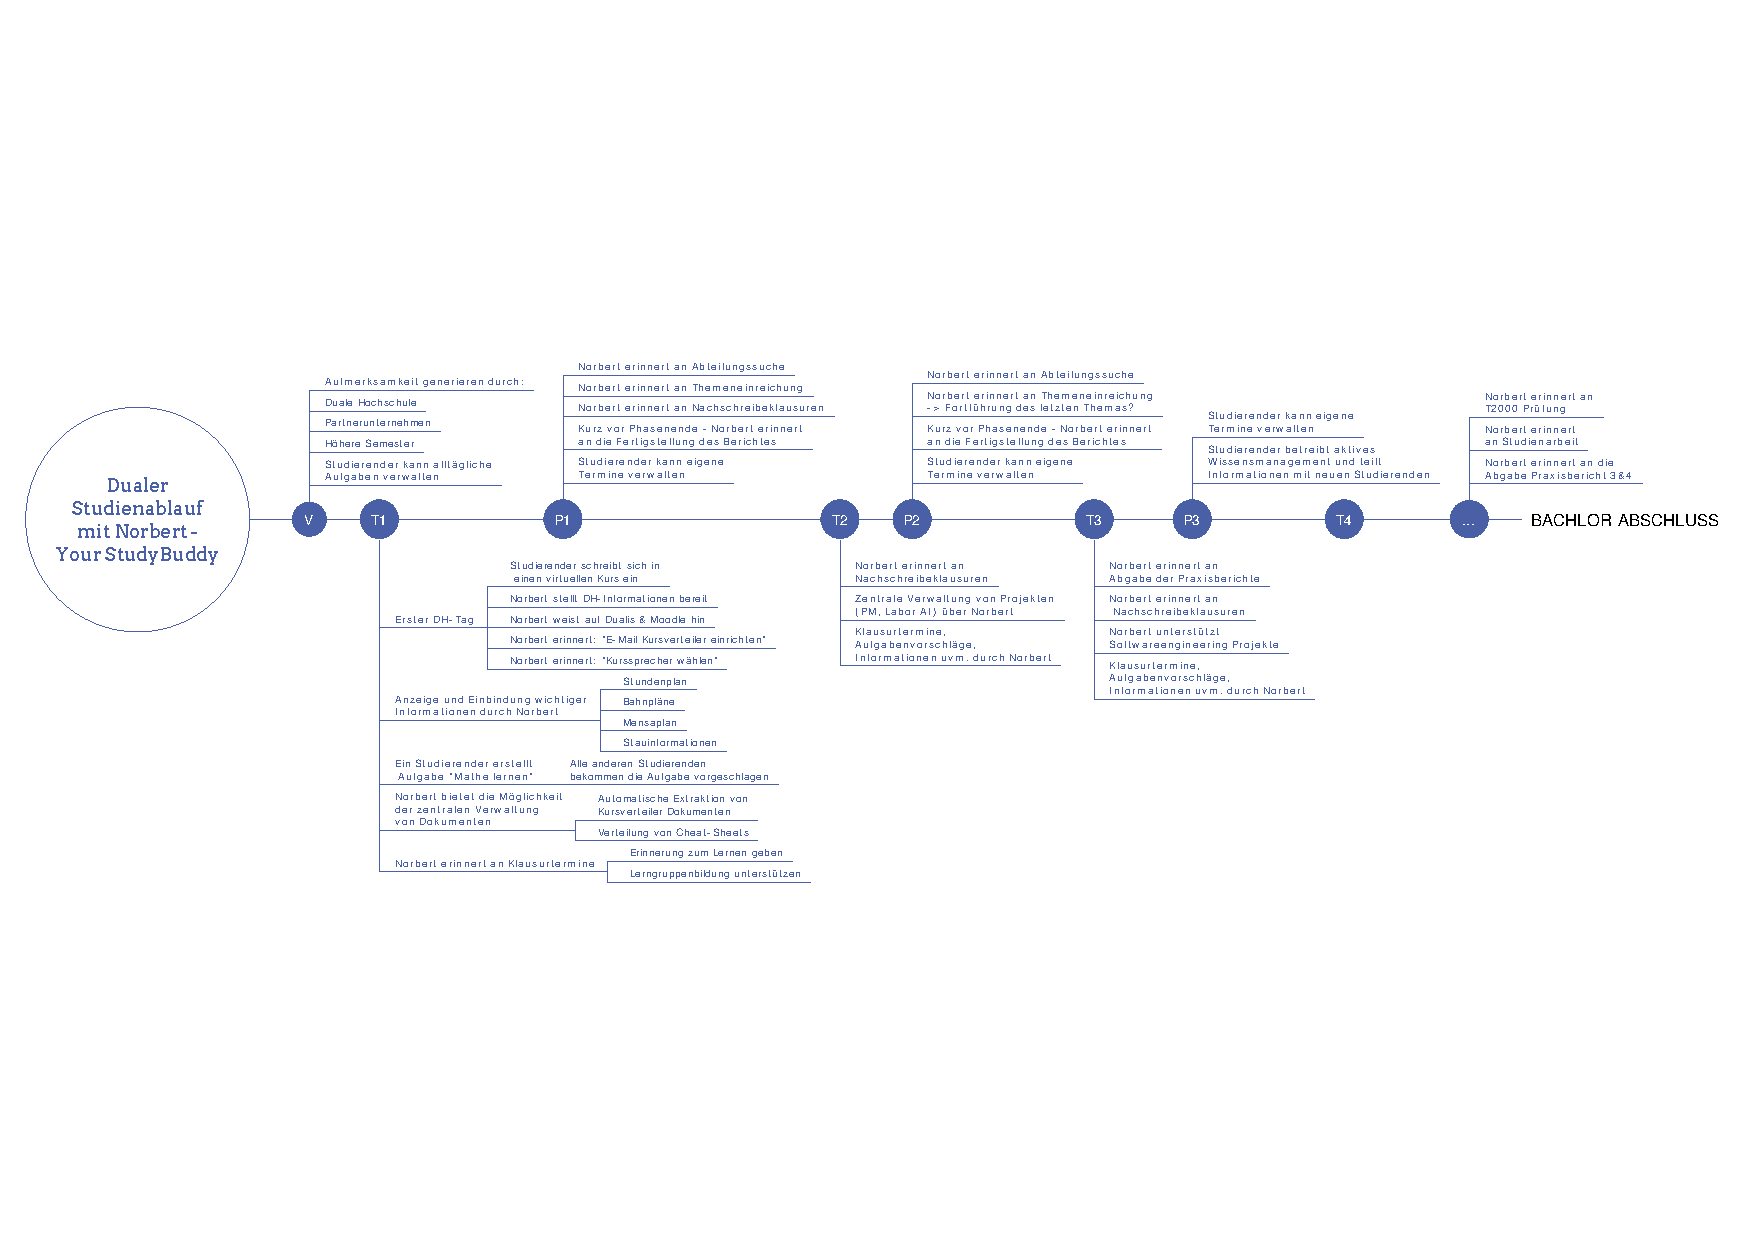
\includegraphics[scale=0.75]{images/timeline.pdf}
	\end{figure}

\end{landscape}
\newpage

\section{Norbert - Wie unterscheidet er sich von anderen Lösungen}

